\documentclass[tikz, border=4pt]{standalone}
\usepackage{tikz}
\usepackage[compat=1.1.0]{tikz-feynman}
\begin{document}
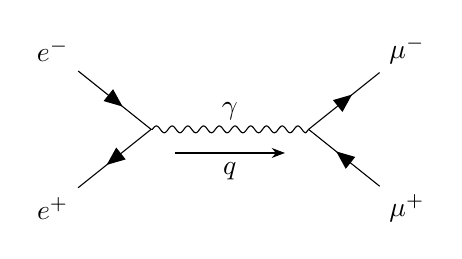
\begin{tikzpicture}[x=1cm, y=1cm]
  \begin{scope}[shift={(0.21,-1.22)}]
  \begin{feynman}
    \vertex (i1) at (0,1) {\(e^-\)};
    \vertex (i2) at (0,-1) {\(e^+\)};
    \vertex (a) at (1.25,0);
    \vertex (b) at (3.25,0);
    \vertex (f1) at (4.5,1) {\(\mu^-\)};
    \vertex (f2) at (4.5,-1) {\(\mu^+\)};
    \diagram* {
      (i1) -- [fermion] (a) -- [fermion] (i2),
      (a) -- [photon, edge label=\(\gamma\), momentum'=\(q\)] (b),
      (f2) -- [fermion] (b) -- [fermion] (f1),
    };
  \end{feynman}
  \end{scope}
\end{tikzpicture}
\end{document}
